\chapter{Contributions}\label{chap:tra}

\section{Présentation de l'outil \kwacceleo{}}\label{sec:acc}

Acceleo est un générateur de code Open Source développé par \kwobeo{} et la fondation Eclipse. \kwacceleo{} permet de générer du code, à partir de modèles basés sur le framework EMF (\cf{} \cite{emf}), en mettant en œuvre l'approche Model Driven Architecture (MDA). Le générateur \kwacceleo{} est une implémentation de la norme de l'OMG pour les transformations de modèle vers texte (Model to Text : M2T \cf{} section \ref{sec:m2t}).

\subsection{Fonctionnement}

Comme la plupart des générateurs de code, \kwacceleo{} propose un système basé sur les templates : les fichiers à générer peuvent être écrits avec des éléments statiques mêlés à des éléments dynamiques.

\subsubsection{Les Modules}

Dans \kwacceleo{}, un Module est une unité de génération amenée a être utilisée par le générateur. Un générateur est donc une agrégation de Modules. Un Module est paramétré par un ou plusieurs \textit{DSL}\footnote{Domain Specific Language} (M2) afin de pouvoir proposer les fonctionnalités associées, qui permettent notamment de parcourir chaque élément du Modèle. Chaque Module est composé d'un ou plusieurs templates. Un template a pour rôle de générer du code d'après un ou plusieurs paramètres.

\begin{figure}[htb]
  \centering
  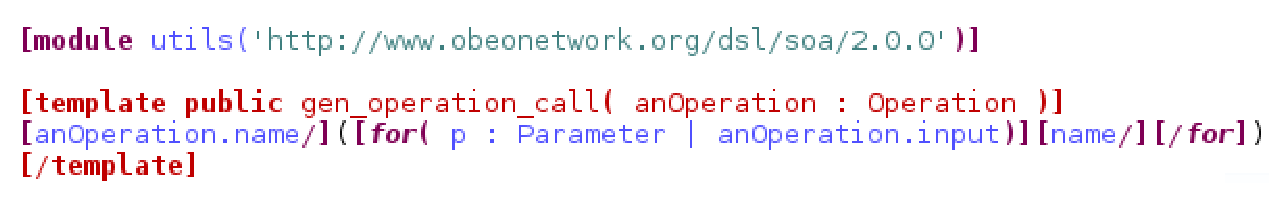
\includegraphics[scale=0.6]{img/screen_template.eps}
  \caption{Exemple de fichier Module dans \kwacceleo{}}
  \label{fig:acc_module}
\end{figure}

L'utilisation des templates est rendue très intuitive grâce au langage conçu pour \kwacceleo{} : Par défaut, le texte écrit dans un template est recopié tel-quel dans le fichier qui sera généré en sortie. Afin d'insérer du contenu dynamique (base de la génération) dans le texte du template, \kwacceleo{} utilise les balises \guim{\textbf{[}} (ouvrantes) et \guim{\textbf{/]}} (fermantes). Ces balisent permettent d'insérer un certain nombre d'instructions, comme la récupération d'un attribut d'un élément du Modèle fourni en entrée, mais aussi des opérations conditionnelles ou des boucles de traitement.

Par convention, chaque Module concerne un ou plusieurs aspects de la génération. Un Module peut également être dédié à la génération d'un type de fichier en particulier.


% Peut être une tite capture d'écran ici (Je m'en charge)

\subsubsection{Les Queries}

Les Modules permettent de décomposer la génération du code en plusieurs sous-parties réutilisables. Ils utilisent donc les templates pour générer un même type de contenu texte à partir de différents éléments du même type.\\
Cependant, dans certains cas, il est nécessaire d'exécuter des opérations moins triviales (modification d'une chaine, calcul, etc\dots).\\
Les \textit{Queries} interviennent alors comme un moyen de factoriser ces opérations non-triviales dans une base commune, différente des templates.
Une des spécificités des \textit{Queries} par rapport aux templates est que ces dernières mettent en cache leur résultat. Ainsi, si une \textit{Query} est appelée deux fois avec les mêmes paramètres, celle-ci ne sera pas re-calculée et se contentera de retourner le résultat obtenu précédement. Cette fonctionnalité est donc très utile pour l'appel répétitif d'opérations (même basiques), ou le stockage de variables globales.\\
Les Queries permettent donc de structurer le générateur, en séparant la génération de texte et les autres traitements et calculs. Par convention, les générations de texte sont traitées dans des templates, tandis que les opérations plus complexes (modification de chaine, parcours d'éléments, stockage de variable statique) ou répétitives sont déportées dans des \textit{Queries}.

\begin{figure}[htb]
  \centering
  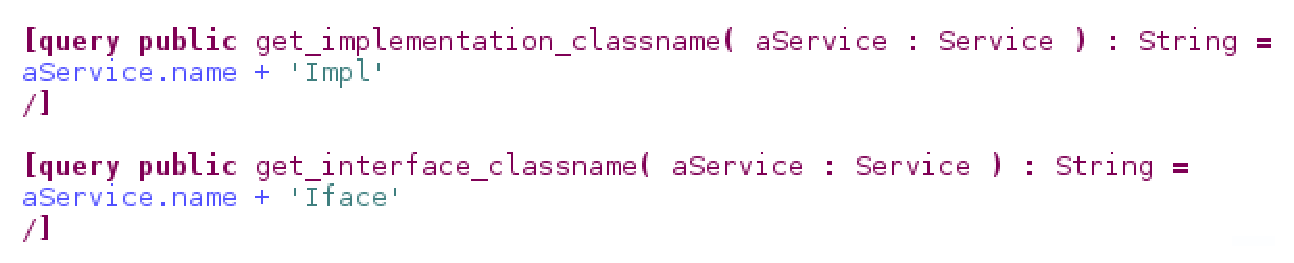
\includegraphics[scale=0.6]{img/screen_query.eps}
  \caption{Exemple de Queries dans \kwacceleo{}}
  \label{fig:acc_module}
\end{figure}

\subsubsection{Les Services}

Les Services peuvent être vus comme une extension des Queries. Là où les opérations exécutables des Query se limitent à actions basiques (définies avec \textit{Ocl}\footnote{Ocl : Object Constraint Language}). Les Services reposent sur le principe qu'il est possible d'appeler du code Java depuis une Query via des invocations de méthodes. Cela permet d'effectuer des opérations complexes ou bien de stocker un certain nombre d'informations via du code Java. Ces informations restent récupérables depuis les templates pendant toute la durée de la génération de code.

\subsubsection{Les balises \guim{Code Utilisateur}}

L'expérience d'\kwobeo a montré qu'un objectif de 100\% de code généré n'est, dans la majorité des cas, ni atteignable ni souhaitable.
En d'autres termes, un code généré sera rarement complet. C'est pourquoi \kwacceleo fournit un système très simple permettant de définir des zones de \guim{Code Utilisateur} au sein d'un Template. Ainsi, l'utilisateur peut apporter des modifications ou ajouts dans les fichiers générés. Si ces modifications ont été effectuées à l'intérieur d'une zone \guim{Code Utilisateur}, ces dernières ne seront pas affectées si les fichiers sont générés à nouveau.
De telles zones peuvent être insérées au sein d'un Template en utilisant de simples balises \guim{\textit{\textbf{[protected]}}}.
\\
Des études ont déjà été effectuées afin de chercher le moyen d'assurer l'efficacité et la maintenabilité d'un code généré, notamment le design pattern \textit{Generation Gap} \cite{gen_gap}.

% Ici un schema ?
\begin{figure}[htb]
  \centering
  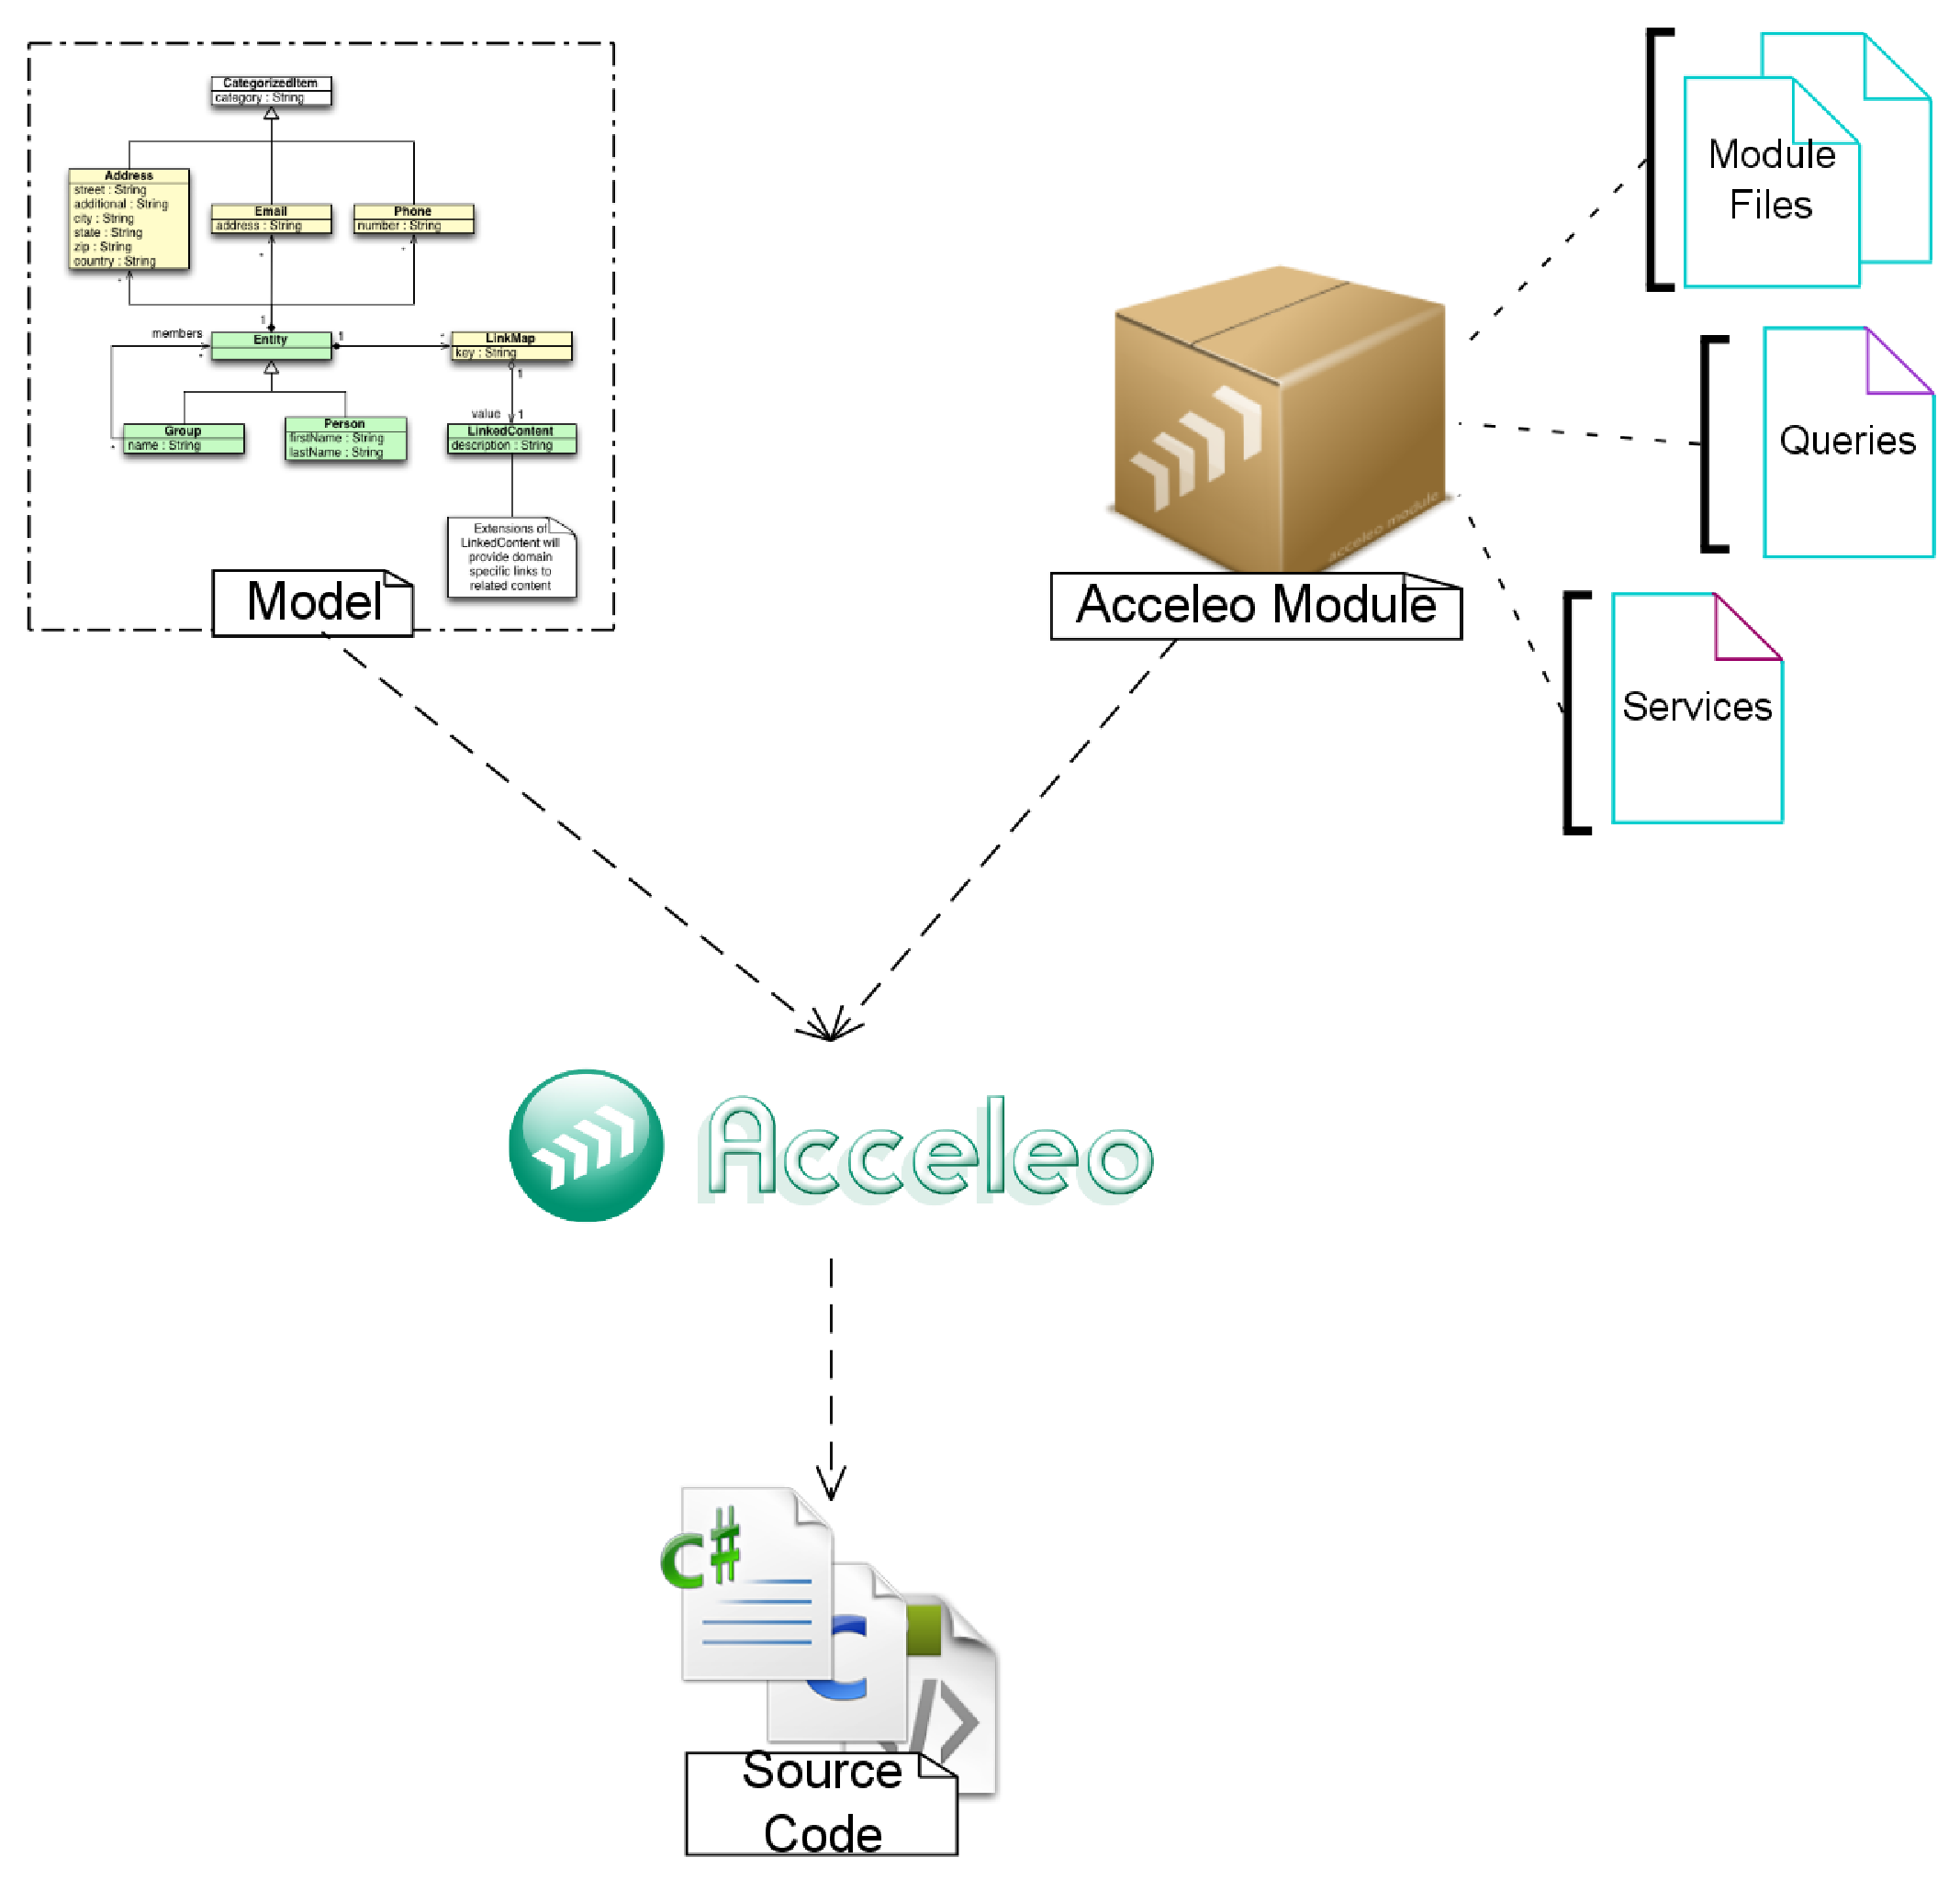
\includegraphics[scale=0.29]{img/acceleo_scheme.eps}
  \caption{Fonctionnement d'Acceleo}
  \label{fig:acceleo}
\end{figure}

%\subsection{Déploiement}
%
%Afin de gérer le déploiement des différents générateurs de %code, 

% Causer du système de menus/plugins/etc
\clearpage

\inputnp{4a_Travaux_Entity} 
\inputnp{4b_Travaux_SOA}
\inputnp{4c_Travaux_Cinematic}
\inputnp{4d_Deploiement}
